% !TeX root = RJwrapper.tex
\title{pdp: An R Package for Constructing Partial Dependence Plots}
\author{by Author One}

\maketitle

\abstract{%
Complex nonparametric models---like neural networks, random forests, and
support vector machines---are more common than ever in predictive
analytics, especially when dealing with large observational databases
that don't adhere to the strict assumptions imposed by traditional
statistical techniques (e.g., multiple linear regression which assumes
linearity, homoscedasticity, and normality). Unfortunately, it can be
challenging to understand the results of such models and explain them to
management. Partial dependence plots offer a simple solution. Partial
dependence plots are low-dimensional graphical renderings of the
prediction function \(\widehat{f}\left(\boldsymbol{x}\right)\) so that
the relationship between the outcome and predictors of interest can be
more easily understood. These plots are especially useful in explaining
the output from black box models. In this paper, we introduce \pkg{pdp},
a general R package for constructing partial dependence plots.
}

\hypertarget{introduction}{%
\subsection{Introduction}\label{introduction}}

\textbf{Note:} This is an updated version of the original R Journal
article.

\citet{harrison-1978-hedonic} were among the first to analyze the
well-known Boston housing data. One of their goals was to find a housing
value equation using data on median home values from \(n = 506\) census
tracts in the suburbs of Boston from the 1970 census; see
\citet[Table IV]{harrison-1978-hedonic} for a description of each
variable. The data violate many classical assumptions like linearity,
normality, and constant variance. Nonetheless,
\citeauthor{harrison-1978-hedonic}---using a combination of
transformations, significance testing, and grid searches---were able to
find a reasonable fitting model (\(R^2 = 0.81\)). Part of the payoff for
there time and efforts was an interpretable prediction equation which is
reproduced in Equation\textasciitilde{}\eqref{eqn:boston}.
\begin{equation}
\label{eqn:boston}
\begin{aligned}
\widehat{\log\left(MV\right)} &= 9.76 + 0.0063 RM^2 + 8.98\times10^{-5} AGE - 0.19\log\left(DIS\right) + 0.096\log\left(RAD\right) \\
  & \quad - 4.20\times10^{-4} TAX - 0.031 PTRATIO + 0.36\left(B - 0.63\right)^2 - 0.37\log\left(LSTAT\right) \\
  & \quad - 0.012 CRIM + 8.03\times10^{-5} ZN + 2.41\times10^{-4} INDUS + 0.088 CHAS \\
  & \quad - 0.0064 NOX^2
\end{aligned}
\end{equation}

Nowadays, many supervised learning algorithms can fit the data
automatically in seconds---typically with higher accuracy. (We will
revisit the Boston housing data in
Section\textasciitilde{}\ref{sec:boston}.) The downfall, however, is
some loss of interpretation since these algorithms typically do not
produce simple prediction formulas like
Equation\textasciitilde{}\eqref{eqn:boston}. These models can still
provide insight into the data, but it is not in the form of simple
equations. For example, quantifying predictor importance has become an
essential task in the analysis of ``big data'', and many supervised
learning algorithms, like tree-based methods, can naturally assign
variable importance scores to all of the predictors in the training
data.

While determining predictor importance is a crucial task in any
supervised learning problem, ranking variables is only part of the story
and once a subset of ``important'' features is identified it is often
necessary to assess the relationship between them (or subset thereof)
and the response. This can be done in many ways, but in machine learning
it is often accomplished by constructing \dfn{partial dependence plots}
(PDPs); see \citet{friedman-2001-greedy} for details. PDPs help
visualize the relationship between a subset of the features (typically
1-3) and the response while accounting for the average effect of the
other predictors in the model. They are particularly effective with
black box models like random forests and support vector machines.

Let \(\boldsymbol{x} = \left\{x_1, x_2, \dots, x_p\right\}\) represent
the predictors in a model whose prediction function is
\(\widehat{f}\left(\boldsymbol{x}\right)\). If we partition
\(\boldsymbol{x}\) into an interest set, \(\boldsymbol{z}_s\), and its
compliment,
\(\boldsymbol{z}_c = \boldsymbol{x} \setminus \boldsymbol{z}_s\), then
the ``partial dependence'' of the response on \(\boldsymbol{z}_s\) is
defined as \begin{equation}
\label{eqn:avg_fun}
  f_s\left(\boldsymbol{z}_s\right) = E_{\boldsymbol{z}_c}\left[\widehat{f}\left(\boldsymbol{z}_s, \boldsymbol{z}_c\right)\right] = \int \widehat{f}\left(\boldsymbol{z}_s, \boldsymbol{z}_c\right)p_{c}\left(\boldsymbol{z}_c\right)d\boldsymbol{z}_c,
\end{equation} where \(p_{c}\left(\boldsymbol{z}_c\right)\) is the
marginal probability density of \(\boldsymbol{z}_c\):
\(p_{c}\left(\boldsymbol{z}_c\right) = \int p\left(\boldsymbol{x}\right)d\boldsymbol{z}_s\).
Equation\textasciitilde{}\eqref{eqn:avg_fun} can be estimated from a set
of training data by \begin{equation}
\label{eqn:pdf}
\bar{f}_s\left(\boldsymbol{z}_s\right) = \frac{1}{n}\sum_{i = 1}^n\widehat{f}\left(\boldsymbol{z}_s,\boldsymbol{z}_{i, c}\right),
\end{equation} where \(\boldsymbol{z}_{i, c}\)
\(\left(i = 1, 2, \dots, n\right)\) are the values of
\(\boldsymbol{z}_c\) that occur in the training sample; that is, we
average out the effects of all the other predictors in the model.

Constructing a PDP \eqref{eqn:pdf} in practice is rather
straightforward. To simplify, let \(\boldsymbol{z}_s = x_1\) be the
predictor variable of interest with unique values
\(\left\{x_{11}, x_{12}, \dots, x_{1k}\right\}\). The partial dependence
of the response on \(x_1\) can be constructed as follows:

\begin{algorithm}
\begin{enumerate}
  \item For $i \in \left\{1, 2, \dots, k\right\}$:
  \begin{enumerate}
    \item Copy the training data and replace the original values of $x_1$ with the constant $x_{1i}$.
    \item Compute the vector of predicted values from the modified copy of the training data.
    \item Compute the average prediction to obtain $\bar{f}_1\left(x_{1i}\right)$.
  \end{enumerate}
  \item Plot the pairs $\left\{x_{1i}, \bar{f}_1\left(x_{1i}\right)\right\}$ for $i = 1, 2, \dotsc, k$.
\end{enumerate}
\caption{A simple algorithm for constructing the partial dependence of the response on a single predictor $x_1$. \label{alg:pdp}}
\end{algorithm}

Algorithm\textasciitilde{}\ref{alg:pdp} can be quite computationally
intensive since it involves \(k\) passes over the training records.
Fortunately, the algorithm can be parallelized quite easily (more on
this in Section\textasciitilde{}\ref{sec:computational}). It can also be
easily extended to larger subsets of two or more features as well.

Limited implementations of Friedman's PDPs are available in packages
\CRANpkg{randomForest} \citep{randomForest-pkg} and \CRANpkg{gbm}
\citep{gbm-pkg}, among others; these are limited in the sense that they
only apply to the models fit using the respective package. For example,
the \code{partialPlot} function in \pkg{randomForest} only applies to
objects of class \code{"randomForest"} and the \code{plot} function in
\pkg{gbm} only applies to \code{"gbm"} objects. While the
\pkg{randomForest} implementation will only allow for a single
predictor, the \pkg{gbm} implementation can deal with any subset of the
predictor space. Partial dependence functions are not restricted to
tree-based models; they can be applied to any supervised learning
algorithm (e.g., generalized additive models and neural networks).
However, to our knowledge, there is no general package for constructing
PDPs in R. For example, PDPs for a conditional random forest as
implemented by the \code{cforest} function in the \CRANpkg{party} and
\CRANpkg{partykit} packages; see \citet{party-pkg} and
\citet{partykit-pkg}, respectively. The \CRANpkg{pdp} \citep{pdp-pkg}
package tries to close this gap by offering a general framework for
constructing PDPs that can be applied to several classes of fitted
models.

The \CRANpkg{plotmo} package \citep{plotmo-pkg} is one alternative to
\pkg{pdp}. According to \citeauthor{plotmo-pkg}, \pkg{plotmo} constructs
``a poor man's partial dependence plot.'' In particular, it plots a
model's response when varying one or two predictors while holding the
other predictors in the model constant (continuous features are fixed at
their median value, while factors are held at their first level). These
plots allow for up to two variables at a time. They are also less
accurate than PDPs, but are faster to construct. For additive models
(i.e., models with no interactions), these plots are identical in shape
to PDPs. As of \pkg{plotmo} version 3.3.0, there is now support for
constructing PDPs, but it is not the default. The main difference is
that \pkg{plotmo}, rather than applying step 1. (a)-(c) in
Algorithm\textasciitilde{}\ref{alg:pdp}, accumulates all the data at
once thereby reducing the number of internal calls to \code{predict}.
The trade-off is a slight increase in speed at the expense of using more
memory. So, why use the \pkg{pdp} package? As will be discussed in the
upcoming sections, \pkg{pdp}:

\begin{itemize}
  \item contains only a few functions with relatively few arguments;
  \item does \underline{not} produce a plot by default;
  \item can be used more efficiently with \code{"gbm"} objects (see Section~\ref{sec:computational});
  \item produces graphics based on \CRANpkg{lattice} \citep{lattice-pkg}, which are more flexible than base R graphics;
  \item defaults to using false color level plots for multivariate displays (see Section~\ref{sec:multi});
  \item contains options to mitigate the risks associated with extrapolation (see Section~\ref{sec:computational});
  \item has the option to display progress bars (see Section~\ref{sec:computational});
  \item has the option to construct PDPs in parallel (see Section~\ref{sec:computational});
    \item is extremely flexible in the types of PDPs that can be produced (see Section~\ref{sec:prediction}),
\end{itemize}

Several additional packages have been developed in recent years that
provide similar functionality to \pkg{pdp}, such as the \CRANpkg{iml}
package \citep{iml-pkg}.

PDPs can be misleading in the presence of substantial interactions
\citep{goldstein-peeking-2015}. To overcome this issue
\citeauthor*{goldstein-peeking-2015} developed the concept of
\dfn{individual conditional expectation} (ICE) plots---available in the
\CRANpkg{ICEbox} package. ICE plots display the estimated relationship
between the response and a predictor of interest for each observation.
Consequently, the PDP for a predictor of interest can be obtained by
averaging the corresponding ICE curves across all observations. In
Section\textasciitilde{}\ref{sec:prediction}, it is shown how to obtain
ICE curves using the \pkg{pdp} package. It is also possible to display
the PDP for a single predictor with \pkg{ICEbox}; see
\code{?ICEbox::plot.ice} for an example. \pkg{ICEbox} only allows for
one variable at a time (i.e., no multivariate displays), though color
can be used effectively to display information about an additional
predictor. The ability to construct centered ICE (c-ICE) plots and
derivative ICE (d-ICE) plots is also available in \pkg{ICEbox}; c-ICE
plots help visualize heterogeneity in the modeled relationship between
observations, and d-ICE plots help to explore interaction effects.

Many other techniques exist for visualizing relationships between the
predictors and the response based on a fitted model. For example, the
\CRANpkg{car} package \citep{fox-car-2011} contains many functions for
constructing \dfn{partial-residual} and \dfn{marginal-model} plots.
\dfn{Effect displays}, available in the \CRANpkg{effects} package
\citep{fox-effects-2003}, provide tabular and graphical displays for the
terms in parametric models while holding all other predictors at some
constant value---similar in spirit to \pkg{plotmo}'s marginal model
plots. However, these methods were designed for simpler parametric
models (e.g., linear and generalized linear models), whereas
\pkg{plotmo}, \pkg{ICEbox}, and \pkg{pdp} are more useful for black box
models (although, they can be used for simple parametric models as
well).

\section{Constructing PDPs in R}

The \pkg{pdp} package is useful for constructing PDPs for many classes
of fitted models in R. PDPs are especially useful for visualizing the
relationships discovered by complex machine learning algorithms such as
a random forest. The latest stable release is available from
\href{https://cran.r-project.org/package=pdp}{CRAN}. The development
version is located on GitHub: \url{https://github.com/bgreenwell/pdp}.
Bug reports and suggestions are appreciated and should be submitted to
\url{https://github.com/bgreenwell/pdp/issues}. The two most important
functions exported by \pkg{pdp} are:

\begin{itemize}
  \item \code{partial}
  \item \code{plotPartial}
\end{itemize}

The \code{partial} function evaluates the partial dependence
\eqref{eqn:pdf} from a fitted model over a grid of predictor values; the
fitted model and predictors are specified using the \code{object} and
\code{pred.var} arguments, respectively---these are the only required
arguments. If \code{plot = FALSE} (the default), \code{partial} returns
an object of class \code{"partial"} which inherits from the class
\code{"data.frame"}; put another way, by default, \code{partial} returns
a data frame with an additional class that is recognized by the
\code{plotPartial} function. The columns of the data frame are labeled
in the same order as the features supplied to \code{pred.var}, and the
last column is labeled
\code{yhat}\footnote{There is one exception to this. When a function supplied via the \code{pred.fun} argument returns multiple predictions, the second to last and last columns will be labeled \code{yhat} and \code{yhat.id}, respectively (see Section~\ref{sec:prediction}).}
and contains the values of the partial dependence function
\(\bar{f}_s\left(\boldsymbol{z}_s\right)\). If \code{plot = TRUE}, then
\code{partial} makes an internal call to \code{plotPartial} (with fewer
plotting options) and returns the PDP in the form of a \pkg{lattice}
plot (i.e., a \code{"trellis"} object). \strong{Note:} it is recommended
to call \code{partial} with \code{plot = FALSE} and store the results;
this allows for more flexible plotting, and the user will not have to
waste time calling \code{partial} again if the default plot is not
sufficient.

The \code{plotPartial} function can be used for displaying more advanced
PDPs; it operates on objects of class \code{"partial"} and has many
useful plotting options. For example, \code{plotPartial} makes it
straight forward to add a LOESS smooth, or produce a 3-D surface instead
of a false color level plot (the default). Of course, since the default
output produced by \code{partial} is still a data frame, the user can
easily use any plotting package he/she desires to visualize the
results---\CRANpkg{ggplot2} \citep{ggplot2-pkg}, for instance (see
Section\textasciitilde{}\ref{sec:classification} and
Section\textasciitilde{}\ref{sec:prediction} for examples).

\strong{Note:} as mentioned above, \pkg{pdp} relies on \pkg{lattice} for
its graphics. \pkg{lattice} itself is built on top of \CRANpkg{grid}
\citep{grid-pkg}. \pkg{grid} graphics behave a little differently than
traditional R graphics, and two points are worth making (see
\code{?lattice} for more details):

\begin{enumerate}
  \item \pkg{lattice} functions return a \code{"trellis"} object, but do not display it; the \code{print} method produces the actual display. However, due to R's automatic printing rule, the result is automatically printed when using these functions in the command line. If \code{plotPartial} is called inside of \code{source} or inside a loop (e.g., \code{for} or \code{while}), an explicit \code{print} statement is required to display the resulting graph; hence, the same is true when using \code{partial} with \code{plot = TRUE}.
  \item Setting graphical parameters via \code{par} typically has no effect on \pkg{lattice} plots. Instead, \pkg{lattice} provides its own \code{trellis.par.set} function for modifying graphical parameters.
\end{enumerate}

A consequence of the second point is that the \code{par} function cannot
be used to control the layout of multiple \pkg{lattice} (and hence
\pkg{pdp}) plots. Simple solutions are available in packages
\CRANpkg{latticeExtra} \citep{latticeExtra-pkg} and \CRANpkg{gridExtra}
\citep{gridExtra-pkg}. For convenience, \pkg{pdp} imports the
\code{grid.arrange} function from \pkg{gridExtra} which makes it easy to
display multiple \pkg{grid}-based graphical objects on a single plot
(these include graphics produced using \pkg{lattice} (hence, \pkg{pdp})
and \pkg{ggplot2}). This is demonstrated in multiple examples throughout
this paper.

Currently supported models are described in
Table\textasciitilde{}\ref{tab:models}. In these cases, the user does
not need to supply a prediction function (more on this in
Section\textasciitilde{}\ref{sec:prediction}) or a value for the
\code{type} argument (i.e., \code{"regression"} or
\code{"classification"}). In other situations, the user may need to
specify one or both of these arguments. This allows \code{partial} to be
flexible enough to handle many of the model types not listed in
Table\textasciitilde{}\ref{tab:models}; for example, neural networks
from the \CRANpkg{nnet} package \citep{venables-modern-2002}.\% and
projection pursuit regression \citep{friedman-ppr-1981} using the
\code{ppr} function in the \pkg{stats} package.

\begin{table}[!htbp]
  \begin{tabular}{p{4cm}ll}
    \toprule
      Type of model & R package & Object class \\
      \midrule
      Decision tree             & \CRANpkg{C50} \citep{C50-pkg} & \code{"C5.0"} \\
                                & \pkg{party}    & \code{"BinaryTree"} \\
                                & \pkg{partykit} & \code{"party"} \\
                                & \CRANpkg{rpart} \citep{rpart-pkg} & \code{"rpart"} \\
      Bagged decision trees     & \CRANpkg{adabag} \citep{adabag-pkg} & \code{"bagging"} \\
                                & \CRANpkg{ipred} \citep{ipred-pkg} & \code{"classbagg"}, \\ & & \code{"regbagg"} \\
      Boosted decision trees    & \CRANpkg{adabag} \citep{adabag-pkg} & \code{"boosting"} \\
                                & \pkg{gbm}      & \code{"gbm"} \\
                                & \CRANpkg{xgboost} & \code{"xgb.Booster"} \\
      Cubist                    & \CRANpkg{Cubist} \citep{Cubist-pkg} & \code{"cubist"} \\
      Discriminant analysis     & \CRANpkg{MASS} \citep{venables-modern-2002} & \code{"lda"}, \code{"qda"} \\
      Generalized linear model  & \pkg{stats}    & \code{"glm"}, \code{"lm"} \\
      Linear model              & \pkg{stats}    & \code{"lm"} \\
      Nonlinear least squares   & \pkg{stats}    & \code{"nls"} \\
      Multivariate adaptive regression splines (MARS) & \CRANpkg{earth} \citep{earth-pkg} & \code{"earth"} \\
                                & \CRANpkg{mda} \citep{mda-pkg} & \code{"mars"} \\
      Projection pursuit regression & \pkg{stats} & \code{"ppr"} \\
      Random forest             & \pkg{randomForest} & \code{"randomForest"} \\
                                & \pkg{party}        & \code{"RandomForest"} \\
                                & \pkg{partykit} & \code{"cforest"} \\
                                & \CRANpkg{ranger} \citep{ranger-pkg} & \code{"ranger"} \\
      Support vector machine    & \CRANpkg{e1071} \citep{e1071-pkg} & \code{"svm"} \\
                                & \CRANpkg{kernlab} \citep{kernlab-pkg} & \code{"ksvm"} \\
      \bottomrule
  \end{tabular}
  \caption{Models specifically supported by the \pkg{pdp} package. \strong{Note:} for some of these cases, the user may still need to supply additional arguments in the call to \code{partial}.}
  \label{tab:models}
\end{table}

The \code{partial} function also supports objects of class
\code{"train"} produced using the \code{train} function from the
well-known \CRANpkg{caret} package \citep{caret-pkg}. This means that
\code{partial} can be used with any classification or regression model
that has been fit using \pkg{caret}'s \code{train} function; see
\url{http://topepo.github.io/caret/available-models.html} for a current
list of models supported by \pkg{caret}. An example is given in
Section\textasciitilde{}\ref{sec:xgboost}.

Another important argument to \code{partial} is \code{train}. If
\code{train = NULL} (the default), \code{partial} tries to extract the
original training data from the fitted model object. For objects that
typically store a copy of the training data (e.g., objects of class
\code{"BinaryTree"}, \code{"RandomForest"}, and \code{"train"}), this is
straightforward. Otherwise, \code{partial} will attempt to extract the
call stored in \code{object} (if available) and use that to evaluate the
training data in the same environment from which \code{partial} was
called. This can cause problems when, for example, the training data
have been changed after fitting the model, but before calling
\code{partial}. Hence, it is good practice to always supply the training
data via the \code{train} argument in the call to
\code{partial}\footnote{For brevity, we ignore this option in most of the examples in this paper.}.
If \code{train = NULL} and the training data can not be extracted from
the fitted model, the user will be prompted with an informative error
message (this will occur, for example, when using \code{partial} with
\code{"ksvm"} and \code{"xgb.Booster"} objects):

\begin{example}
Error: The training data could not be extracted from object. Please supply
the raw training data using the `train` argument in the call to `partial`.
\end{example}

For illustration, we will use a corrected version of the Boston housing
data analyzed in \citet{harrison-1978-hedonic}; the data are available
in the \pkg{pdp} package (see \code{?pdp::boston} for details). We begin
by loading the data and fitting a random forest with default tuning
parameters and 500 trees:

\begin{Schunk}
\begin{Sinput}
library(randomForest)  # for randomForest, partialPlot, and varImpPlot functions

data(boston, package = "pdp")  # load the (corrected) Boston housing data

# Fit a default random forest to the Boston housing data
set.seed(101)  # for reproducibility
boston.rf <- randomForest(cmedv ~ ., data = boston, importance = TRUE)
varImpPlot(boston.rf)  # Figure 1
\end{Sinput}
\begin{figure}[!htb]

{\centering 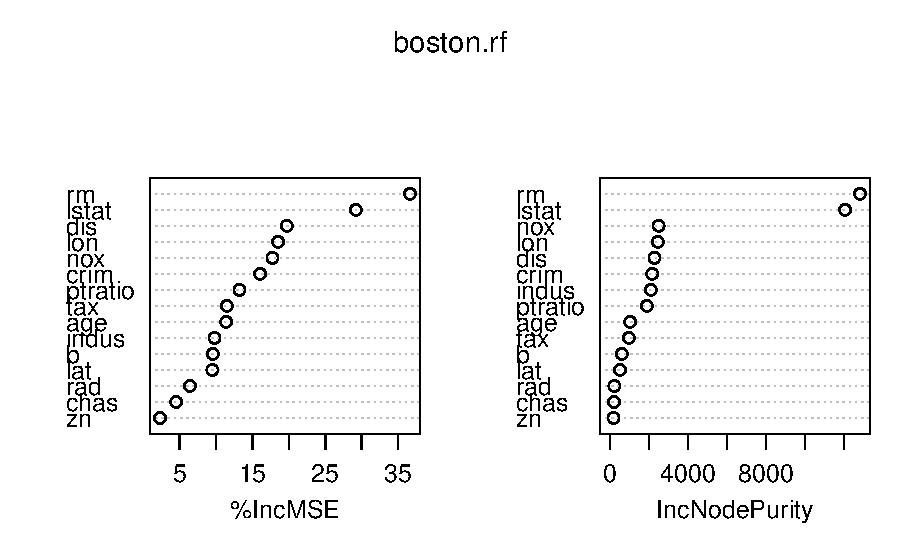
\includegraphics[width=1\linewidth]{greenwell_files/figure-latex/boston-vip-1} 

}

\caption[Dotchart of variable importance scores for the Boston housing data based on a random forest with 500 trees]{Dotchart of variable importance scores for the Boston housing data based on a random forest with 500 trees.}\label{fig:boston-vip}
\end{figure}
\end{Schunk}

The model fit is reasonable, with an \dfn{out-of-bag} (pseudo) \(R^2\)
of 0.89. The variable importance scores are displayed in
Figure\textasciitilde{}\ref{fig:boston-vip}. Both plots indicate that
the percentage of lower status of the population (\code{lstat}) and the
average number of rooms per dwelling (\code{rm}) are highly associated
with the median value of owner-occupied homes (\code{cmedv}). The
question then arises, ``What is the nature of these associations?'' To
help answer this, we can look at the partial dependence of \code{cmedv}
on \code{lstat} and \code{rm}, both individually and together.

\bibliography{greenwell.bib}

\address{%
Author One\\
Affiliation\\%
line 1\\ line 2\\
%
\url{https://journal.r-project.org}\\%
\textit{ORCiD: \href{https://orcid.org/0000-0002-9079-593X}{0000-0002-9079-593X}}\\%
\href{mailto:author1@work}{\nolinkurl{author1@work}}%
}
